\documentclass{article}
\usepackage{amsmath}
\usepackage{amssymb}
\usepackage{amsfonts}
\usepackage[T1]{fontenc}
\usepackage{bm}
\usepackage{array}
\usepackage{graphicx}
\usepackage[utf8]{inputenc}
\usepackage{minted}


\begin{document}
In all of the above the decoder is simply the oposite of the encoder.
\section{Experiment}
First, just to check that stuff works, the convolutional autoencoder identical to
the convolutional layer of the policy network in the Nature paper was used.
It worked very well, but the feature dimension was 3136.
Also the Q learning from this was in fact slower,
altough that could be due to the fact that the policy network was smaller
as it was just 2 FC layers.

The encoder was the following one:
\begin{minted}[mathescape, linenos]{python}
self.encoder = nn.Sequential(
    nn.Conv2d(n_input_channels, 32, kernel_size=8, stride=4, padding=0),
    nn.ReLU(),
    nn.Conv2d(32, 64, kernel_size=4, stride=2, padding=0),
    nn.ReLU(),
    nn.Conv2d(64, 64, kernel_size=3, stride=1, padding=0),
    nn.ReLU(),
    nn.Flatten(),
)

\end{minted}

In any case, we are looking for the smallest possible feature spaces
and this feels like it is not it.

\section{Experiment}
Next the following encoder was tried:

\begin{minted}[mathescape, linenos]{python}
This has the feature dimension of 288, but the number of parameters seems
to be too small for it to work.
self.encoder = nn.Sequential(
    nn.Conv2d(n_input_channels, 8, kernel_size=8, stride=4, padding=0),
    nn.ReLU(),
    nn.Conv2d(8, 16, kernel_size=8, stride=2, padding=0),
    nn.ReLU(),
    nn.Conv2d(16, 32, kernel_size=4, stride=1, padding=0),
    nn.ReLU(),
    nn.Conv2d(32, 32, kernel_size=2, stride=1, padding=0),
    nn.ReLU(),
    nn.Flatten(),
)
\end{minted}

and this looks like:
\begin{figure}[htpb]
		\centering
		
\includegraphics[width=1.0\textwidth]{../../latent_only/ae_resulting_images_features_dim_288_small.png}
		\caption{../../latent_only/ae_resulting_images_features_dim_288_small}
\end{figure}

The idea then was to try a network with a larger number of parameters,
but which will yield the same feature dimension.

\section{Experiment}
The following network:
\begin{minted}[mathescape, linenos]{python}
if self._features_dim == 288:
    self.encoder = nn.Sequential(
        nn.Conv2d(n_input_channels, 16, kernel_size=8, stride=4, padding=0),
        nn.ReLU(),
        nn.Conv2d(16, 16, kernel_size=8, stride=2, padding=0),
        nn.ReLU(),
        nn.Conv2d(16, 32, kernel_size=4, stride=1, padding=0),
        nn.ReLU(),
        nn.Conv2d(32, 32, kernel_size=2, stride=1, padding=0),
        nn.ReLU(),
        nn.Flatten(),
    )

\end{minted}

and it clearly didn't work:
\begin{figure}[htpb]
		\centering
		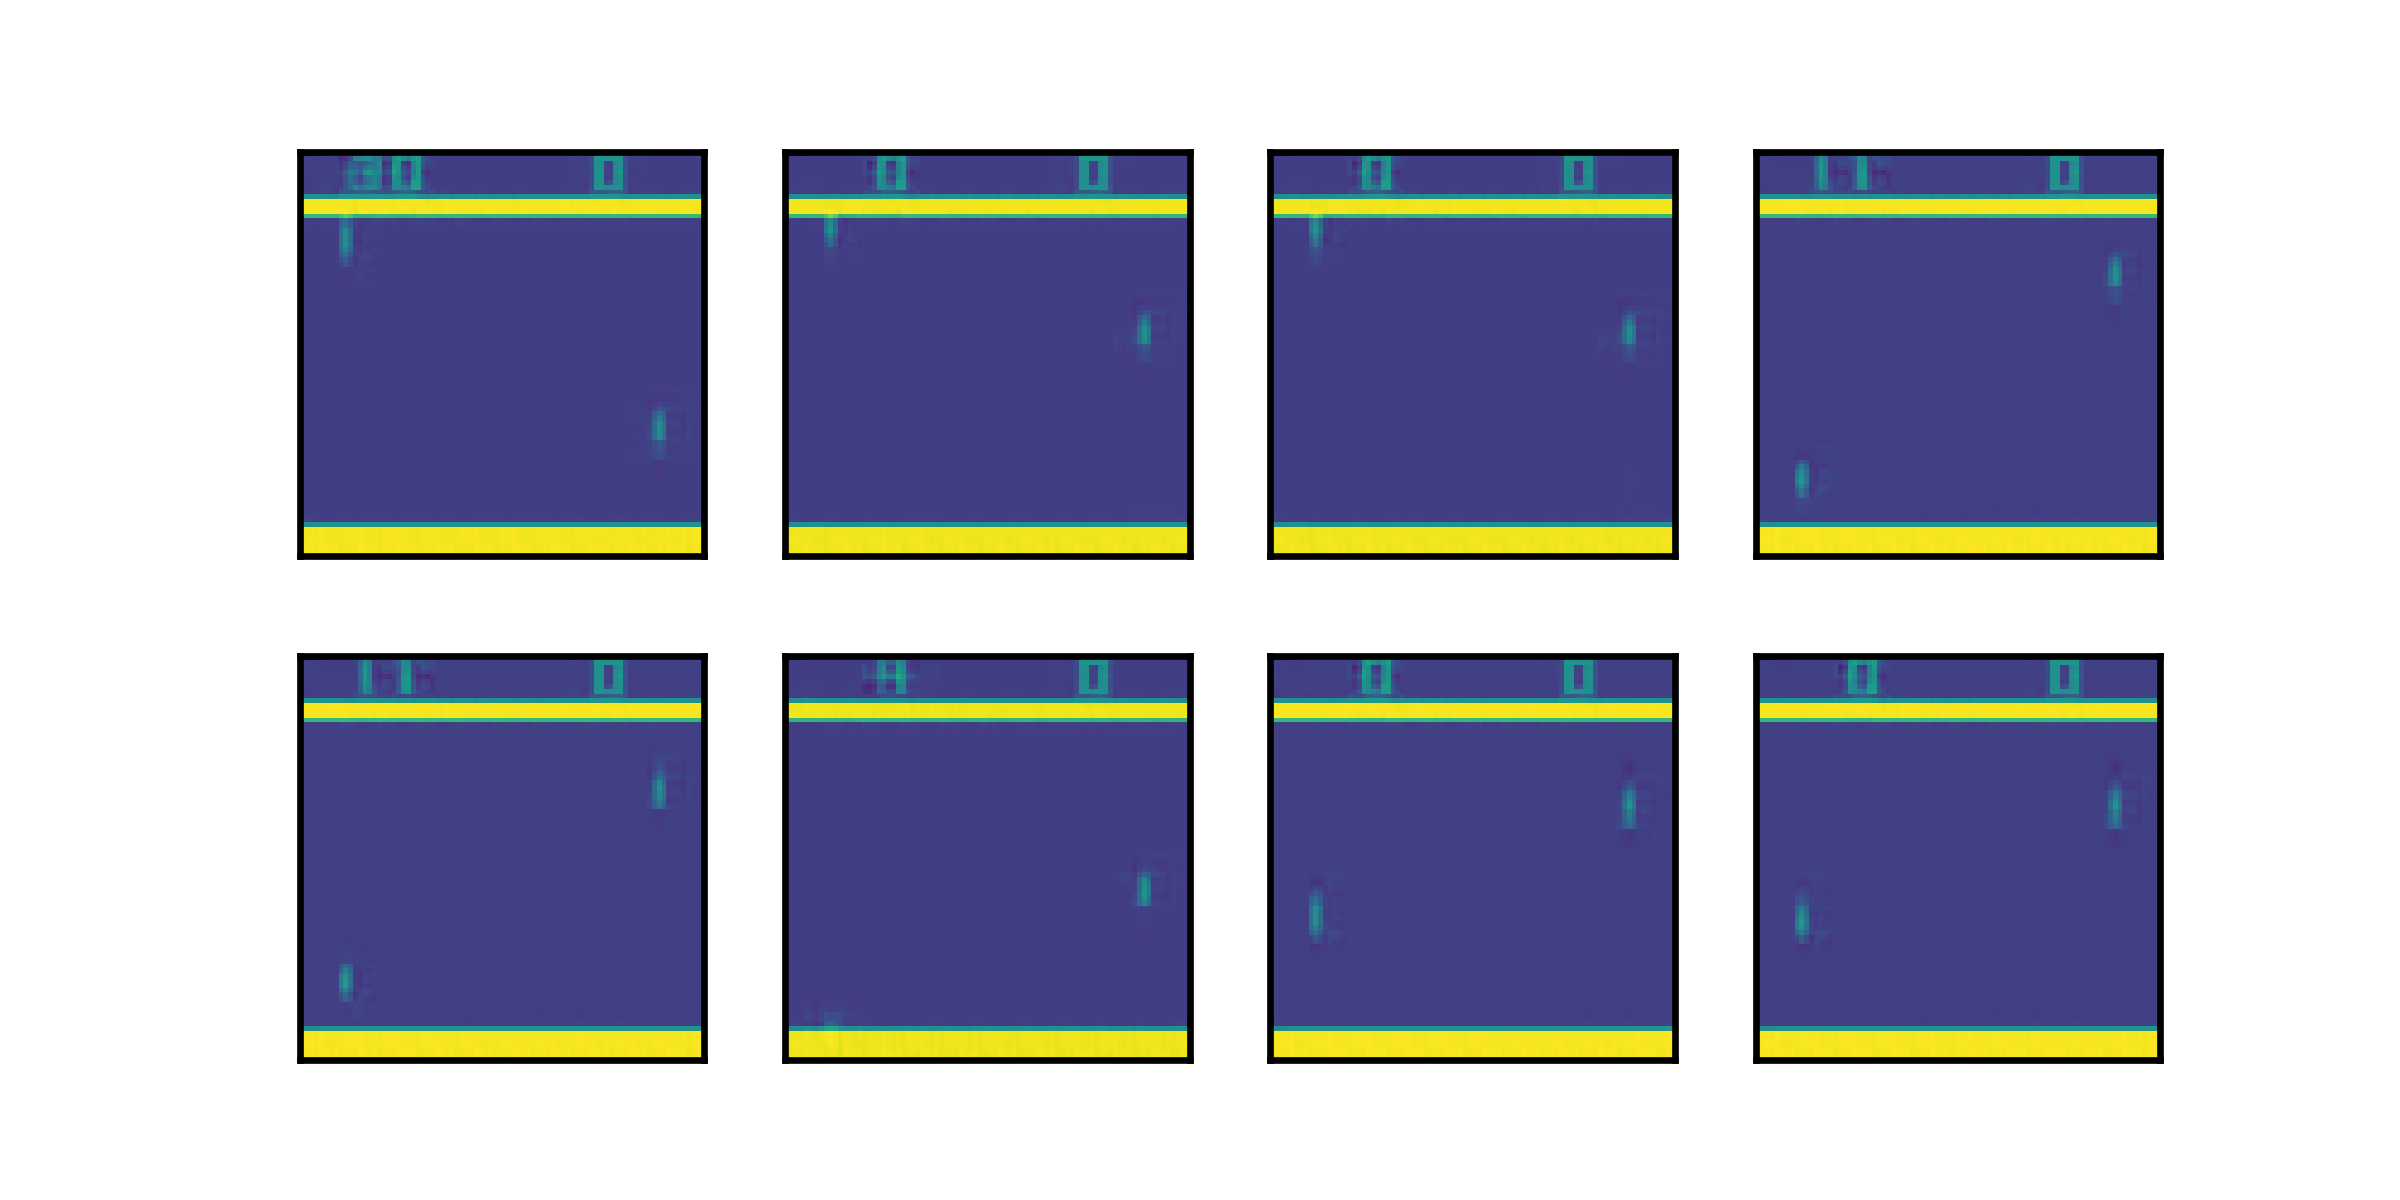
\includegraphics[width=1.0\textwidth]{../../latent_only/ae_resulting_images_features_dim_288_slightly_bigger.png}
		\caption{}
		\label{fig:}
\end{figure}

\end{document}
